\definecolor{lightgray}{rgb}{.9,.9,.9}
\definecolor{darkgray}{rgb}{.4,.4,.4}
\definecolor{purple}{rgb}{0.65, 0.12, 0.82}

\lstdefinelanguage{JavaScript}{
  keywords={typeof, new, true, false, catch, function, return, null, catch, switch, var, if, in, while, do, else, case, break},
  keywordstyle=\color{blue}\bfseries,
  ndkeywords={class, export, boolean, throw, implements, import, this},
  ndkeywordstyle=\color{darkgray}\bfseries,
  identifierstyle=\color{black},
  sensitive=false,
  comment=[l]{//},
  morecomment=[s]{/*}{*/},
  commentstyle=\color{purple}\ttfamily,
  stringstyle=\color{red}\ttfamily,
  morestring=[b]',
  morestring=[b]"
}

\lstset{
   language=JavaScript,
   backgroundcolor=\color{lightgray},
   extendedchars=true,
   basicstyle=\footnotesize\ttfamily,
   showstringspaces=false,
   showspaces=false,
   numbers=left,
   numberstyle=\footnotesize,
   numbersep=9pt,
   tabsize=2,
   breaklines=true,
   showtabs=false,
   captionpos=b
}



\chapter{Evaluation}

The previous chapters outlined our approach to feature extraction and visualization and demonstrated an implementation of it. The following two sections will evaluate the solution both from a technical standpoint and from different user standpoints, taking into consideration the three main use cases that were presented initially; Network Administrator, Researcher and Professor.
\section{Performance Evaluation}
Before we go into a qualitative evaluation of the features implemented within DDoSGrid, we first wanted to assess the solution's technical quality. This is important since our initial requirements stated that we want to support large PCAP files and that our front end should work on a wide range of browsers and devices.
\subsection{Back End}
For the actual decoding and mining procedure we found no comparable tools that we could use to benchmark against. Therefore, we searched for the largest attack trace on the internet with the hypothesis that if this set can be analyzed in a sensible amount of time, our solution could be used for large files. The largest file we found was 4.4 gigabytes in size and provided by the "The U.S. National CyberWatch Mid-Atlantic Collegiate Cyber Defense Competition (MACCDC)". This is a cyber defense challenge for university students where they can learn to deal with such attacks in a realistic setting \cite{maccdc}.
Our solution was able to provide all the features outlined in the following case studies in two minutes and 57 seconds. We think that this is a reasonable time since it includes the visualizations and therefore no further time is required for analysis or parsing.
\subsection{Front End}\label{frontendevaluation}
Regarding the front end, we wanted to ensure that all the current best practises in web development are met and that the application works well on constrained devices and networks. To test this, we used Lighthouse, an open source tool provided by Google. This tool allowed us to assess the web application with respect to its SEO optimization, performance, accessibility and compliance of progressive web standards \cite{lighthouse}.
\begin{figure}
    \centering
    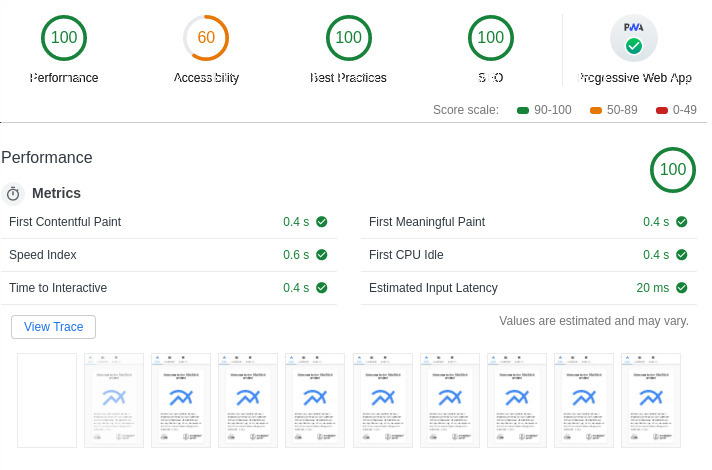
\includegraphics[width=12cm]{images/lighthouse.jpeg}
    \caption{Lighthouse report of the DDoSGrid front end}
    \label{fig:lightouse}
\end{figure}
As we can see in \ref{fig:lightouse} we were able to achieve good performance, even under a simulated 3G device with constrained CPU. DDoSGrid also follows all the best practises suggested by Google and fully complies as a Progressive Web Application, which means that browsers prompt the user to install the application to the home screen. An area that could be improved is the accessibility of the tool.

\section{Case Study \#1: Network Administrator}
Let us suppose that a network operator is in charge of investigating a DDoS attack that targeted the underlying infrastructure of a business. The operator's objective is to get a better idea of the type and characteristics of the attack. For that, different kinds of visualizations are a useful source to write a report on the attack, thus providing insights about possible countermeasures. For the scenario, we assume that the operator has a PCAP file containing information about the multi-vector attack, which consisted of a port scan and a SYN-flood attack. Marty describes that network security professionals are often only given minutes to present their report to non-technical audiences \cite{appliedsecurityvisualization}. For this reason, reducing the incident to easily understandable but important facts and numbers are significant tasks in this scenario.

The operator simply supplies the PCAP file, a name and a description for it and starts the upload process. Due to the size and intensity of today's DDoS attacks it is safe to assume that their captures may be multiple gigabytes in size. Both the analysis and the uploading procedure have been implemented to scale well, even for large file sizes. This means that one could run the application locally without requiring powerful hardware due to the sequential data processing. Once the upload and analysis processes have finished, the user receives a desktop notification to remind them that they can use the data set on the platform.
Once the analysis is finished, elicited and calculated metrics are presented to the operator, informing them about general statistics of the attack, e.g. the attack's duration. These metrics can serve as the base of the report. For example, in one quick glance the number of destination ports that were targeted can be seen. In a very simple report, the operator could list this number and suggest an appropriate solution. To further illustrate the targeted ports example, the suggestion of implementing a DMZ could be made. 

To help the operator find attack patterns, the analyzed data set can be opened on the dashboard tab of the application. Opening multiple data sets at once is also possible, so the operator can compare a packet capture from regular network traffic to that of the attack to find possible weaknesses in the network. On the dashboard page a tile is displayed for each data set containing the possible visualization types grouped by attack type. This grouping allows to observe the data set under different perspectives which were written for specific attack behaviours. This allows to identify attack vectors, i.e. which attack types have been used on the target. Elaborating on the aforementioned example of comparing regular traffic to attack traffic, the same visualization can be opened for both data sets resulting in easy spotting of anomalies. Figure  \ref{fig:datasettilesop} presents a proposed visualization containing a data set from regular traffic on the right side and a data set of traffic under attack on the left side, both displayed using the same graph. As one can see, the destination ports on the left hand side show that a large number of ports have received traffic, compared to the right hand side.
Once weaknesses or interesting behavior is found, the operator can derive measurements to be taken in order to minimize attack risks in the future. To support such proposals it is possible to save the created dashboards and restore them once the operator needs to make a proposal to an executive. For reporting purposes, the operator may also export a single diagram as a PNG or the whole setup as a PDF file. This functionality is further described in \ref{casestudyeducation}. We outlined before how one can compare different data sets on the same chart type and how one can use different diagrams to look for different attack types in the same data set. All of these items, including the metrics computed for each data set, can be flexibly arranged in a grid. The operator can also enlarge certain items to suit their presentation. All of these features allow the network operator to create meaningful results. 

\begin{figure}[]
    \centering
    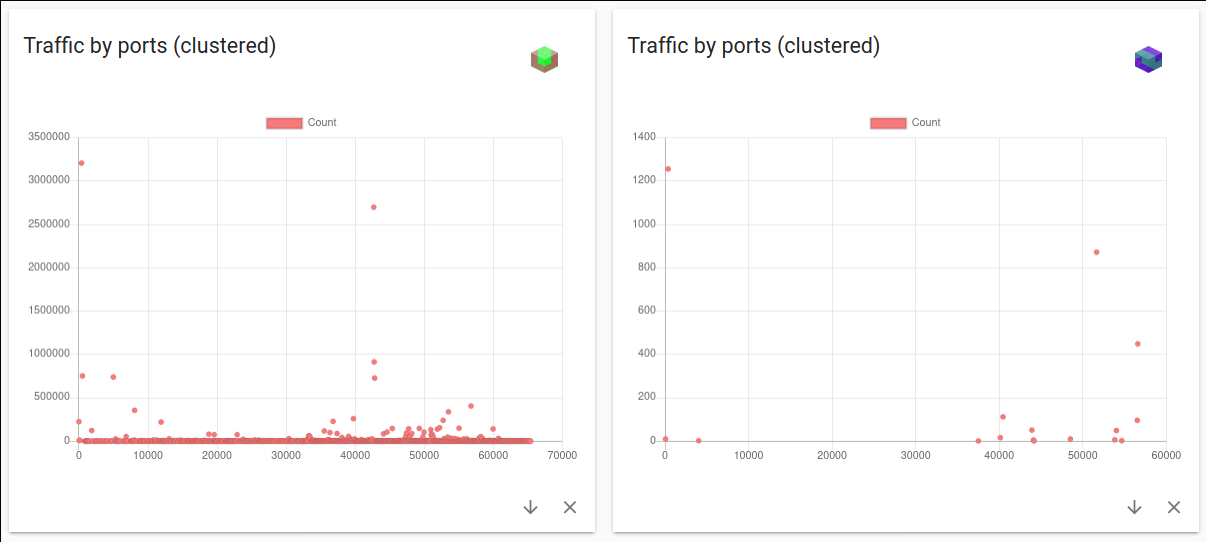
\includegraphics[width=15cm]{images/evaluation_different_datasets_same_visualization.png}
    \caption{Features from two data sets rendered on the same chart. The left diagram originates from a recording of an attack, while the right diagram displays regular network traffic.}
    \label{fig:datasettilesop}
\end{figure}
So far, only one visualization illustrating the number of traffic received in destination ports was shown.
Marty argues that such kind of visualization simplifies the understanding of specific types of DDoS attacks, remarking that the limitations of said visualizations need to be kept in mind. Rendering destination ports can lead to common problems when visualizing network security-related incidents, namely the source-destination confusion \cite{appliedsecurityvisualization}. The destination port can represent either incoming or outgoing packets. This distorts the visualization, since incoming TCP packets of established connections will seem to have a random destination port. Our solution helps combating this issue since the actual visualization is written by someone who wants to understand the attack pattern. Given that the developer is aware of this issue, it would be easy to integrate a warning message or propose a solution. The solution to the actual problem would be to filter only the incoming packets from not-yet established connections, which can be done during the capturing stage or later when performing the analysis. Experiments conducted by using the implemented prototype in \ref{chapDesign} prove that it would be even possible to apply such a filter directly in our application. This would allow for a nice complementation of using tcpdump or Wireshark to do initial pre-processing where one usually works with filters. The filters used in Wireshark or tcpdump could then be used in our application, so that it can be used solely for visualizing and reporting data.
The presented visualization shows traffic by destination port which allows to detect possible portscans and flooding attacks to a certain port. Other visualizations have not been shown for the sake of keeping this case study compact, however it is important to note that once an operator knows about the attack type, they can then use this finding to discover other information such as possible sources of the attack.
Following, a brief enumeration of the other existing visualizations concludes this case study. This is not only important to know in terms of what information a network operator can extract right now with our implementation but also because it proves the point that our solution is capable to visualize different features from any OSI layer in a scalable manner.

 \begin{enumerate}
     \item For each data set the network operator can see important network metrics such as number of packets received or number of ports being targeted. This is an important basis so that one can use it as a direction for which visualization to consider. For example, if the user immediately sees that a large number of different TCP ports is being targeted, it would make sense to look at the destination port visualization shown before.
     \item Relation of traffic received as IPv4- and IPv6-packets can be inspected using a Pie Chart.
     \item The five sources contributing the most packets, their originating prefixes and ASN is shown on a Pie Chart.
     \item The 100 sources contributing the most packets, aggregated by country where their prefix was announced from can be rendered on a world map. This allows to quickly see where traffic might originate from.
     \item For TCP and UDP traffic there are two visualizations, the first one simple shows the 20 ports that received the most traffic on a Bar Chart. For an overview over all ports there is a visualization showing traffic received over all destination ports on a Scatter Plot. To make this plot more readable, the destination ports are aggregated into buckets. This allows to have an overview over the traffic and identify attacks like Portscan attacks.
     \item A Pie Chart visualization showing the proportion of connection states of all TCP packets allows to see if there was a SYN-flood attack. In an attack situation, it becomes apparent that there are proportionately more packets in connection setup state than in other states.
     \item For the final layer, the application layer, the network operator can inspect the usage of HTTP verbs and endpoints on a Pie Chart. This allows the detection of HTTP-based attacks. For example, if the network operator sees that most HTTP requests were directed to \textit{/search.php}, this could indicate that this is a demanding request which might be abused by attackers.
 \end{enumerate}{}



\section{Case Study \#2: Education} \label{casestudyeducation}
Let us assume that a professor in an educational institute wants to efficiently communicate the behaviour of an attack by visualizing its attack pattern. This case study will consider a SYN flood attack, which is a type of DDoS attack represented by a host being flooded with TCP connection requests, that may stem from a spoofed source.
Available network capture files from actual DDoS attacks might contain too much noise or even a multi-vector attack, which could hinder the goal of explaining one specific attack dynamic. In this case, the professor can obtain a network capture by either performing an actual attack in a laboratory environment or by using a tool, e.g. DDoS\_log\_sim \cite{ddoslogsim} to generate a network capture with the desired noise level. The format of the capture would be a PCAP file, which is compatible with our application. PCAP is a common file format and supported by popular tools such as tcpdump and Wireshark.
Now that the capture file is ready, the professor can upload it on the \textit{Data sets} page of our application. This is done by clicking the plus button in the lower right corner and supplying additional information such as a name and description which will be persisted as well. This is easy to work with since the professor could leave all network captures stored on the server and still distinguish between them by reading the description and names. For example, they could upload another capture file with a different attack pattern for a different audience and they could easily distinguish between them. This is also supported by generating an avatar from the SHA256 hash of the file content. This makes it easy to distinguish between data sets just by glancing at the icon. Once the file is uploaded and the analysis is performed, the user will be notified of a successful completion through a desktop notification. Now the professor can open that data set on the visualizations page or upload another data set. An example would be the data set with the same attack pattern but different parameters generated by the DDoS simulator.
Once all desired data sets are opened on the dashboard, the professor can then open specific visualizations to show the characteristics of the different attack types. The visualizations available for the data sets have been written with a specific attack in mind, but they can also be used even if no attack is contained in the data set. This grouping into attack categories should make it as easy as possible to open the right visualizations. The opened data sets, the available visualizations, and their respective avatars are shown in Figure \ref{fig:datasettiles}

\begin{figure}
    \centering
    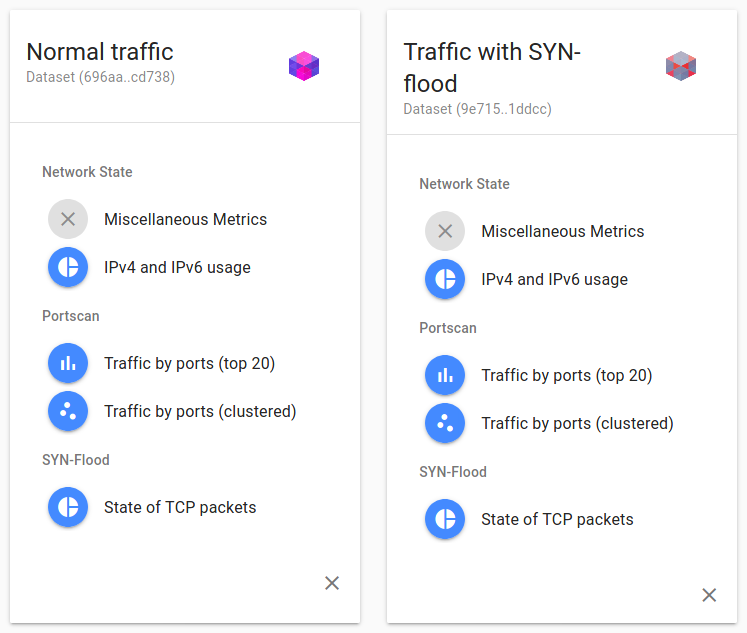
\includegraphics[width=13cm]{images/evaluation-dataset-tiles.png}
    \caption{Two different data sets opened on the visualizations page.}
    \label{fig:datasettiles}
\end{figure}
As mentioned earlier in our example, the professor would be interested in a SYN-flood visualization and would therefore open the pie-chart visualization in the SYN-Flood category. This will open a new tile which briefly explains what is being displayed using its title and description elements. This tile will show the same avatar as its originating data set tile to visually distinguish to which data set this visualization belongs. Using this visualization, the professor can show that a large number of packets are in the (active) connection setup state of a TCP connection which clearly shows the attack pattern of a SYN flood state. This can be seen in Figure \ref{fig:synfloodpiechart}. Now that the professor has a visualization of the attack pattern, they can contrast this by showing either the same visualization for different traffic or a different visualization for the same data set. This way, they can contrast the attack with normal behaviour, making clear that this is sometimes not a trivial task. It will also serve to show that there are no other attacks and that it is in fact a SYN-flood attack.

\begin{figure}
    \centering
    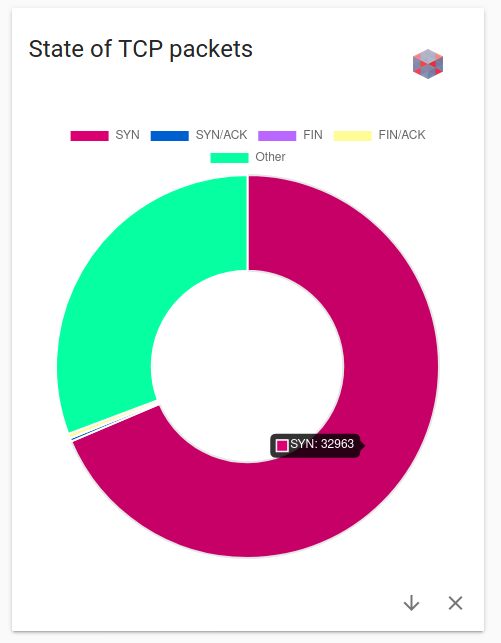
\includegraphics[width=8cm]{images/evaluation-synflood-piechart.png}
    \caption{Piechart showing the state of the TCP connection for each packet using a data set that clearly contained a SYN-flood attack}
    \label{fig:synfloodpiechart}
\end{figure}

In addition to opening and closing data sets and visualizations, the professor can also rearrange the tiles to make connections and differences between tiles more clear. Further, they may filter based on the originating data set, which allows to dynamically highlight certain information during the presentation. Once a satisfying arrangement of tiles is created, the professor has different options of presenting their setup. Firstly, the setup can be saved in their browser cache and restored at later stage. This method of presentation has the advantage of keeping the visualization's interactivity, such as detailed numbers of "SYN" packets upon hovering the cursor on the pie-chart,as shown in figure \ref{fig:synfloodpiechart}. 
The saving and  restoring functionality is available in a Speed-Dial menu at the bottom right corner. For saving a setup, a name has to be provided, while for restoring a setup, the desired setup has to be chosen from a list.
Secondly, the professor can export each visualization by clicking the arrow-down button on each tile. This will render the diagram as a static PNG with transparent background, so that it could be used in presentations or papers.
The third option would be to generate a PDF file based on the current dashboard that was created and download it. This functionality is also available in the lower-right corner.
We can compare our solution to the visualization feature of WireShark which we deem to be a popular alternative.
As one can see in figure \ref{fig:synvisualizationwireshark} it is possible to plot the same data set by solely using WireShark. However, there are a few key differences; firstly, the IO-Graph from WireShark only gives the possibility to plot packets using time on the x-axis and frequency on the y-axis. It is however possible to have different lines for different filters and to configure the line's styles. In any case, the filters need to be written manually; for example we would write a filter like "tcp.flags == 0x02" to show the packets in connection-setup state. We would need to do this analogously for each other state, which can be cumbersome since it requires knowledge about the protocol's implementation. With our solution, the user receives a similar graph without having to know about how the connection states are actually implemented in the protocol. Additionally, the fact that WireShark plots over time may be too detailed to achieve an abstract picture of the attack pattern. This can be improved by increasing the interval for each step on the x-axis.
Once one is satisfied with the configuration of the IO-Graph by supplying filters, colors, scaling and a time interval, one can view, modify and export the graph as a PDF. We think that these are all properties that hold for our solution as well, however with our solution, a user can save this setup for later usage and compare it with other data sets or with other graphs. Nevertheless, WireShark provides interesting features that would be beneficial to apply to our solution as well. This covers the interactive scaling of the graph, changing the interval, dynamically adjusting colors and a graph that plots frequency over time. We deem that all of these features would be technically feasible to implement using our approach. It has to be noted that doing things interactively may come at the price of losing the ability to instantly render the visualization, since different processing has to be applied to the files that can be of varying sizes.

\begin{figure}[]
    \centering
    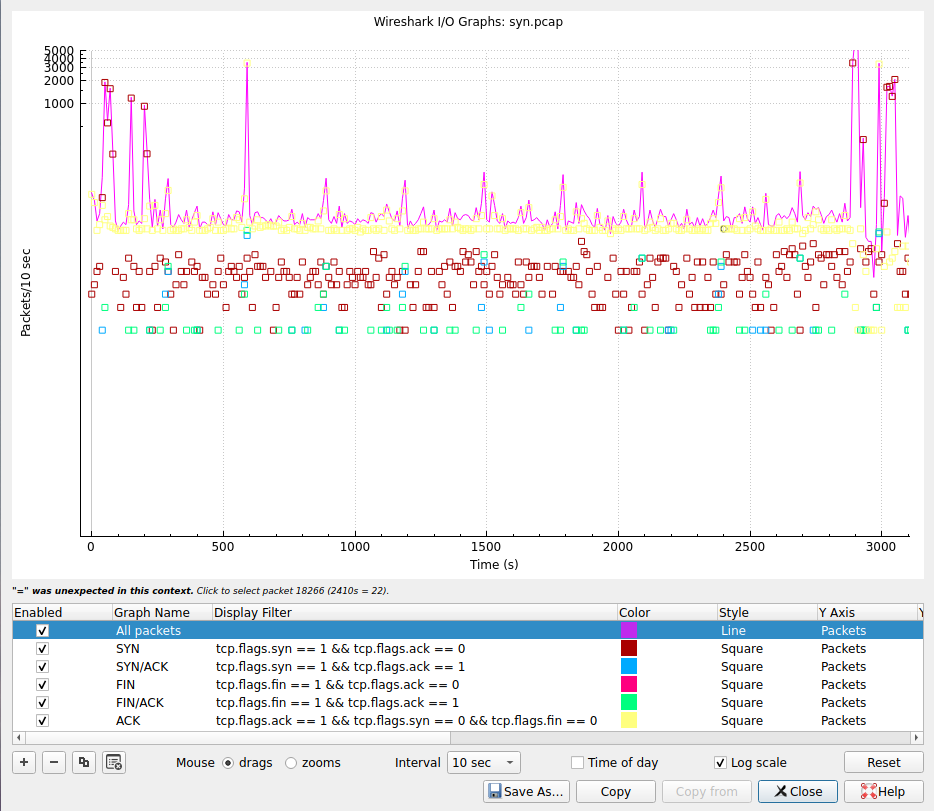
\includegraphics[width=10cm]{images/evaluation_wireshark_iograph_synflood.png}
    \caption{Plotting the same data set using WireShark IO Graph with custom filters}
    \label{fig:synvisualizationwireshark}
\end{figure}

\section{Case Study \#3: Researcher} \label{casestudyresearcher}
In case studies \#1 and \#2 we have described scenarios focusing on using the visualizations for different tasks. This case study describes a scenario where a researcher wants to extend the platform and visualizations according to their needs. There are many possible examples of extending the functionality, since metrics and visualizations are often very context dependent. For example when a researcher has the task of computing an experimental metric or visualization to analyze a completely novel type of DDoS attack, our solution provides  extendable components to simplify implementing these new features.  We assume that there is a researcher who has already analyzed and explored the attack vector of a network capture but now the goal is to derive other information by exploring different dimensions of the data set. Specifically, the researcher would like to visualize which sources contributed the most packets to inbound traffic. Thus, they extend our tool by implementing a new feature extractor which will aggregate the top five source addresses of IPv4 packets. Additionally, the data set should be enhanced with additional information by enriching it with sources other than the actual capture file. For example, they could use a BGP routing table to derive the prefix that the source IPv4 addresses belonged to.

To start, the template file of a feature extractor is duplicated and registered in the interface of the miner package. To do so, a new file \textit{miner/miners/TopNSourceHostsByTraffic.js} with the content as shown in listing \ref{lst:initialtemplate} has to be created.
Initially, we only have a class that inherits from an abstract miner class which contains many convenience methods, e.g. for writing JSON files and the signaling of these files. As a dependency injection, it receives a packet decoder from which one may observe different packets. These subscriptions should be created in a \textit{setUp} method where one may perform asynchronous operations such as connecting to a database. The last method that will be called once all packets have been decoded, is the \textit{postParsingAnalysis} method which is again asynchronous to allow for asynchronous operations once all packets have been decoded. We will make use of this feature in the next step. At the end of that method, the miner class should call the method of the base class that makes sure that the file is written and that everything is being orchestrated correctly. We can also see that, based on the structure of the final result, the appropriate visualization will be used.


\begin{lstlisting}[caption={Initial content of the newly create Miner},label={lst:initialtemplate}]
const AbstractPcapAnalyser = require('./AbstractPCAPAnalyser')
const analysisName = 'TBD'

class SourceHostsAnalyser extends AbstractPcapAnalyser {
    constructor(parser, outPath) {
        super(parser, outPath);
        this.results = [
          // store interim results here
        ]
    }

    // Setup phase, load additional databases, setup subscriptions and signal completion
    async setUp() {
    }

    // Actual mining function
    // Post-analysis phase, do additional computation with the collected data and write it out
    async postParsingAnalysis() {

        var fileName = `${this.baseOutPath}-${analysisName}.json`
        var fileContent = {
          // Signal and format to visualize as piechart
          piechart: {
            datasets: [{
              backgroundColor: [],
              data: Object.values(this.results)
            }],
            labels: []
          }
        }
        var summary = {
            fileName: fileName,
            attackCategory: 'TBD',
            analysisName: 'TBD',
            supportedDiagrams: ['PieChart']
        }
        return await this.storeAndReturnResult(fileName, fileContent, summary)
    }
}

module.exports = SourceHostsAnalyser

\end{lstlisting}

So far, this miner does not have any packet-related functionality. Therefore, the researcher needs to think about which packets are needed to determine the right abstraction to be used when subscribing. This is necessary, since there are events for different protocols as well as for different levels in the TCP/IP reference model. Since the researcher is only interested in the source addresses of IPv4 packets, he/she needs to set up one subscription and define the feature extraction logic as shown in listing \ref{lst:subscriptions}.

\begin{lstlisting}[caption={Creating a subscription and mining source addresses},label={lst:subscriptions}]
    // ...
    
    async setUp () {
        var handler = this.countIPv4Address.bind(this)
        this.pcapParser.on('ipv4Packet', handler)
    }

    countIPv4Address (ipv4Packet) {
        var srcAddress = ipv4Packet.saddr.addr.join('.')
        var existingEntry = this.results.find(item => item.addr === srcAddress)

        if(existingEntry) {
            existingEntry.count++
        } else {
            this.results.push({ addr: srcAddress, count: 1 })
        }
    }
    // ...
 

\end{lstlisting}

As we can see in listing \ref{lst:subscriptions}, the researcher starts observing the \textit{ipv4Packet} event. As a handler a method is supplied that simply counts how many times one IPv4 address is seen as the source of an IPv4 packet. Of course this will match both inbound and outbound packets, so a previous step where he/she pre-propecesses the PCAP files is necessary. Now the researcher has written a feature miner that simply captures and counts source IPv4 addresses.

\begin{lstlisting}[caption={Initial content of the newly create Miner},label={lst:formattinganalysis}]
    // ...
    
    async postParsingAnalysis() {
        var sortedByCount = this.sortEntriesByCount(this.results)
        var topNentries = this.getTopN(this.results, N)
 
        var fileName = `${this.baseOutPath}-${analysisName}.json`
        var fileContent = {
          // Signal and format to visualize as piechart
            piechart: {
               datasets: [{
                    backgroundColor: [
                        '#D33F49',
                        '#77BA99',
                        '#23FFD9',
                        '#27B299',
                        '#831A49'
                    ],
                   data: this.formatData(topNentries)
                }],
                labels: this.formatLabels(topNentries)
            }
        }
        var summary = {
            fileName: fileName,
            attackCategory: 'Network State',
            analysisName: 'Top 5 sources by traffic',
            supportedDiagrams: ['PieChart']
        }
        return await this.storeAndReturnResult(fileName, fileContent, summary)
    }
 
    formatData (elements) {
        return elements.map(entry => entry.count)
    }
 
    formatLabels (elements) {
        return elements.map(entry => entry.addr)
    }
  
    sortEntriesByCount (elements) {
        elements.sort((a, b) => {
            if (a.count > b.count)
                return -1;
            if (a.count < b.count)
                return 1;
            return 0;
        })
    }
    
    // ...

\end{lstlisting}
In listing \ref{lst:formattinganalysis} it seems as if the researcher has to implement quite a few things, however all that was required to do is to use the analysis result and pass it to the \textit{filecontent} object on line seven. Here there are three things the researcher has to consider. Firstly, he/she has to supply the values for the visualization and the respective labels. The former would be the number of occurrences for each IPv4 address and the latter would be the actual addresses in dotted decimal notation. Finally, the type of chart to be used has to be decided, represented on line 21. To sum up the implementation: First, the five addresses with the highest count are computed, then the output of the miner is formatted and configured in a way that the orchestrating module receives all output in a compatible format.
With the file content prepared and the categorization of the miner defined, the researcher has implemented all required aspects to have the PCAP file visualized. The output of what was implemented can be seen on the left side of figure \ref{fig:firstimplementation}.

\begin{lstlisting}[caption={Initial content of the newly create Miner},label={lst:formatlabels}]
    // ...
    async formatLabels (elements) {
        var addresses = elements.map(entry => entry.addr)
        var result = []
        for(var address of addresses) {
            var { route, origin, country } = await this.whois(address)
            // Format example: 1.2.3.4: 1.2.0.0/16 (AS12345, CH)
            var label = `${address}: ${route} (${origin}, ${country})`
            result.push(label)
        }
        return result
    }
\end{lstlisting}

As one might have noticed, there is no asynchronous logic in the method called once the decoding has finished. This will now become important since the researcher would like to supplement the results with data from a remote WHOIS database. We will not go into detail about how the IP lookup using the WHOIS protocol works but we will show how one can perform asynchronous operations in this part of the life cycle to enrich the data.
To implement the lookups of the source addresses, the labels of the diagram need to be reformatted to include the desired information. The researcher thus changes the \textit{formatLabels} method as shown in listing \ref{lst:formatlabels}, so that it fetches the WHOIS data and returns that for labelling.

The implementation of that method is straightforward, the researcher makes sure that the corresponding prefix, origin AS number and country are retrieved form the WHOIS service. These elements are used along with the source address to create a label for the diagram. Now, the researcher can use any data set found in a database such as DDoSDB.org and derive the additional information using our tool. This final visualization is shown in Figure \ref{fig:firstimplementation} on the right side.

As we saw in the previous paragraphs, the researcher was able to compute and visualize new information from his PCAP file and even integrate other data sources.We think it is important to note that only the newly created file had to be touched. It was not necessary to modify other feature miners, orchestration modules or the front end. Thus it is possible to extend the functionality without modifying existing functionality.

\begin{figure}[]
    \centering
    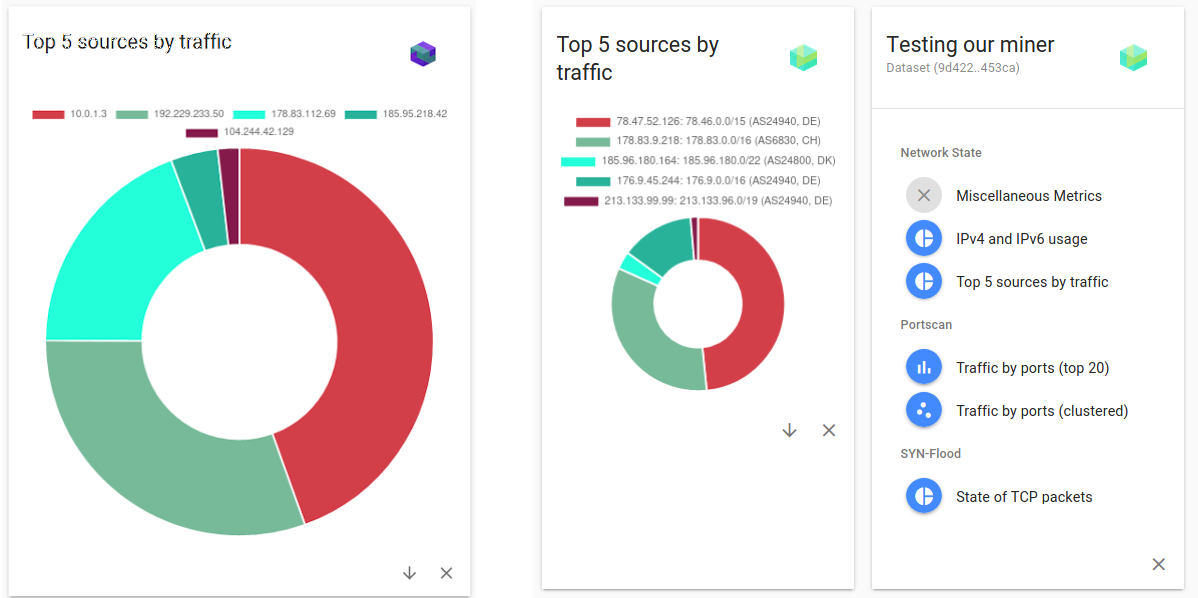
\includegraphics[width=16cm]{images/case-study-researcher-diagrams.png}
    \caption{(i) Resulting diagram after the initial implementation (ii) and after the final improvements}
    \label{fig:firstimplementation}
\end{figure}

\section{Limitations}\label{limitations}% MF: Discussion and Limitations? Add related work together with conclusions as one paragraph
The previous sections have highlighted how the features and architecture provided by our solution can benefit different stakeholders.
While evaluating our solution, a number of limitations and possible improvements were discovered. Since the architecture and design of the system have been written with extensibility in mind, we can safely assume that the following improvements are feasible to implement:
\begin{itemize}

    \item Data source: The application was targeted to use PCAP files, since they are the most common in DDoSDB, a collection of network attacks. A common format that enables similar insights into network traffic flow is NetFlow. In the analysis of possible data sets we found that NetFlow files could also be used as a data source. By complying with the systems architecture consisting of interfaces and a Visitor pattern, one could provide an alternate, Netflow-based data source parser.
    
    \item Data pre-processing: The implementation can be used with network logs from DDoSDB, which are already anonymized. If a raw packet capture is supplied, the same pre-processing is applied. Given certain constraints, such as data privacy laws, this part could be easily extended.
    
    \item Protocol Parsing: 
    In section \ref{networkcapturedecoding} we introduced different protocols and their support by the protocol parser. It would be easy to write additional parsers that handle unsupported protocols. For example, suppose a novel application protocol appears to be used for DDoS attacks. A researcher could use our application and extend it by a decoding module and then perform their analysis by writing a feature extractor.
    
    \item Feature Extractors:
    Creating new analysis processors for the existing PCAP-files would be very easy to write. The user would simply have to register a new visitor and comply with the interfaces or extend them for novel visualizations. For example, assuming that a new application-level protocol would be targeted, the visitor can be registered to be invoked for those types of packets and compute his metrics.
   
    \item Data Integration:
    The system is not integrated with DDoSDB in a fully automated manner due to lack of interfaces. Technically, it would be possible to integrate the uploading  of processed files to DDoSDB or the download such files.
    This also applies for other tools such as DDoS\_log\_sim which does not have a front end yet \cite{ddoslogsim}. It would be quite simple to add a page next to the file upload page where one could configure the generation of the log files.
    
    \item Visualizations
    The part that is easiest to adapt and extend is the set of visualizations. Since the front end was written with a component-based approach, one can easily reuse and change the visualizations. By adhering to the data set, a developer can easily create new components and integrate them into the system without having to know all too much about the systems internals, such as the data processing.
    
    \item Capture Filters
    We have tested prototypes where the user was able to supply a valid filter from tcpdump which would be used during the decoding process. This feature could be integrated into the front end to make it even easier to use tools like Wireshark and tcpdump for pre-processing and then using our platform purely for visualization purposes.
    
    \item Live Captures
    The underlying decoding library supports packet capturing directly from the network interface. This could be integrated into the parser and front end to allow live visualizations.
    
    \item Web Accessibility
    As our front end evaluation indicated, there are different improvements that could be made to the front end to increase its accessibility.
    
    \item User Management
    Currently the application does not differentiate between users. This functionality could be implemented to have administrator and regular users. For example administrators can upload data sets while regular users can only use the dashboard.
    
    \item Time-Based Visualizations
    Results of miners that extract data into time slots can be used in visualizations that can be replayed to simulate the attack either in real time or fast-forwarded.
    
    \item Filters Inside Visualizations
    Due to the extensible nature of our architecture, the visualizations themselves could be adapted to host filters on their own to be set on the dashboard. For example, minimum and maximum thresholds could be set for a port scan to filter out outliers.
    
\end{itemize}
